\subsection{Example}\label{sec:example}
\newcommand{\pone}{$\langle service\_owner=dataset\_owner\rangle$}
\newcommand{\ptwo}{$\langle service\_owner=partner(dataset\_owner) \rangle$}
\newcommand{\pthree}{$\langle service\_owner \neq dataset\_owner AND owner \neq partner(dataset\_owner)$}

\begin{table*}[ht!]
  \def\arraystretch{1.5}
  \centering
  \caption{Anonymization policies}\label{tab:anonymization}



  \begin{tabular}[t]{c|c|l}
    \textbf{Vertex}      & \textbf{Policy} & \policy{subject}{object}{action}{environment}{transformation}                                   \\ \hline
    \vi{1},\vi{2},\vi{3} & $\p{0}$         & \policy{ANY}{dataset}{READ}{ANY}{\tp{0}}                                                        \\
    \vi{4},\vi{6}        & $\p{1}$         & \policy{\pone}{dataset}{READ}{ANY}{\tp{0}}                                                      \\
    \vi{4},\vi{6}        & $\p{2}$         & \policy{\ptwo}{dataset}{READ}{ANY}{\tp{1}}                                                      \\
    \vi{4},\vi{6}        & $\p{3}$         & \policy{\pthree}{dataset}{READ}{ANY}{\tp{2}}                                                    \\
    \vi{5}               & $\p{4}$         & \policy{ANY}{dataset}{READ}{ANY}{\tp{2}}                                                        \\
    \vi{7}               & $\p{5}$         & \policy{$\langle service\_region=``FACILITY"\rangle$}{dataset}{WRITE}{ANY}{\tp{0}}              \\
    \vi{7}               & $\p{6}$         & \policy{$\langle service\_region=``\{CT,NY,NH\}"\rangle$}{dataset}{WRITE}{ANY}{\tp{1}}          \\
    \vi{8}               & $\p{7}$         & \policy{$\langle user\_role=``Connecticut Prison Officer"\rangle$}{dataset} {READ}{ANY}{\tp{0}} \\
    \vi{8}               & $\p{8}$         & \policy{$\langle user\_role=``Partner Prison Officer"\rangle$}{dataset} {READ}{ANY}{\tp{1}}     \\
    \vi{8}               & $\p{9}$         & \policy{$\langle user\_role=``Any"\rangle$}{dataset} {READ}{ANY}{\tp{2}}                        \\
  \end{tabular}

\end{table*}
\begin{table*}[ht!]
  \def\arraystretch{1.5}
  \centering
  \caption{Anonymization levels}\label{tab:levels}
  \begin{tabular}[t]{c|c|l}
    \textbf{\tf{i}} & \textbf{Level} & \textbf{Columns Anonymized}                      \\\hline
    \tp{0}          & Level0         & $anon(\varnothing)$                              \\
    \tp{1}          & level1         & $anon(FIRST\_NAME, LAST\_NAME)$                  \\
    \tp{2}          & level2         & $anon(FIRST\_NAME, LAST\_NAME, IDENTIFIER, AGE)$ \\
  \end{tabular}

\end{table*}

We present an example of pipeline template focusing on policy annotations. The pipeline template consists of five stages, and each stage is annotated with a policy presented in \cref{tab:anonymization}. \hl{Connecticut Prison (CTP) is the service user executing the pipeline. New York Prison and New Hampshire Prison are two partner DOC.}\hl{SPOSTARE NEL SYSTEM MODEL? SI, MA DATA OWNER DIPENDE DAL DATASET, HO MESSO SERVICE USER} We recall that \cref{tab:dataset} shows a sample of our reference dataset.

In the following we will make reference to three different type of anonymization:%\hl{E' GIUSTO USARE}\tf{i}
\hl{? SPOSTIAMO PRIMA?}
\begin{enumerate*}[label=\roman*)]
  \item \emph{level0} (\tp{0}): no anonymization is performed;
  \item \emph{level1} (\tp{1}): the data is partially anonymized, only the first name and last name are anonymized;
  \item \emph{level2} (\tp{2}): the data is fully anonymized: first name, last name, identifier and age are anonymized.
\end{enumerate*}

Let us consider the pipeline template \tChartFunction in \cref{sec:example},
% 1° NODO %
The first stage consists of three parallel vertices (\vi{1}, \vi{2}, \vi{3}) and focuses on data collection.
The policy annotation \p{0} is linked with an empty transformation.
The functional requirement necessitates a URI as input, and the output is the downloaded dataset.

The second stage incorporates a sole vertex (\vi{4}), which merges the three datasets obtained from the previous stages and is associated with three policies (\p{1},\p{2},\p{3}).
The policies are evaluated during the node execution:
%if the service profile matches with the data owner ($owner = ``CTP"$), \p{1} is satisfied and the data is not anonymized (\tf{1});
%if the service profile matches with a partner of the owner ($owner = ``CTP"$), \p{2} is satisfied and the data is partially anonymized (\tf{2});
%if the service profile doesn't match with a partner nor with the owner ($owner = ``CTP"$), \p{3} is satisfied and the data is fully anonymized (\tf{3}).
% 2° NODO %
%he second vertex is responsible for enriching the data.
%The service downloads the dataset from partner facilities and enhances the dataset of the Connecticut facility.
if the service is  by the data owner (\pone), which means that if the service owner is the same as the dataset owner, the dataset is not anonymized (\tp{0}).
if the service is a partner of the data owner (\ptwo), which means that if the service owner is a partner of the dataset owner, the dataset is anonymized level1 (\tp{1}).
if the service is a third party (\pthree), which means that if the service owner is neither the dataset owner nor a partner of the dataset owner, the dataset is anonymized level2 (\tp{2}).
The functional requirement specifies $n$ datasets as input, and the output is the merged dataset.
% 3° NODO %
The third stage, is responsible both for data analysis/statistics and machine learning tasks.
The stage is composed of two alternative vertices respectively \vi{4}, \vi{5}.

Data analytics vertex adopts policies analogous to the second stage. The logic remains consistent:
if the service profile matches with the data owner (\pone), \p{1} is satisfied and the data computation is made on clean data (\tp{0});
if the service profile matches with a partner of the owner (\ptwo), \p{2} is satisfied and the data computation is made on data anonymized level1 (\tp{1});
if the service profile doesn't match with a partner nor with the owner (\pthree), \p{3} is satisfied and the data computation is made on data anonymized level2  (\tp{2}).
The functional requirement specifies a dataset as input, and the output is the computed statistics.
% 4° NODO %
Machine Learning vertex adopts always a level2 anonymization (\p(4)) to prevent personal identifiers from entering into the machine learning algorithm/model (\tp{2}).
The functional requirement specifies a dataset as input, and the output is the trained model or an inference.
% 5° NODO %
The fifth stage manages data storage.
If the service is within the facility itself ($\langle service,region=FACILITY"\rangle$), \p{5} is satisfied, resulting in data anonymization level1 (\tp{1}).
Otherwise, if the service is in a partner region ($\langle service,region={CT,NY,NH}"\rangle$), the data undergo anonymization level2 (\tp{2}).
The functional requirement specifies some\hl{?} data as input, and the output is the URI of the stored data.
% 6° NODO %
The sixth stage is responsible for data visualization.
As stated in policy annotation \p{6}, if the user is member of the facility itself, the data are anonymized level0 (\tp{0}).
If the user is member of a partner facility, the data are anonymized level1 (\tp{2}).
If the user is not member of the facility nor a partner, the data are anonymized level2 (\tp{3}).
The functional requirement specifies a dataset as input, and the output is the visualization of the data.

%In summary, this section has delineated a comprehensive pipeline template. This illustrative pipeline serves as a blueprint, highlighting the role of policy implementation in safeguarding data protection across diverse operational stages.




\begin{figure}[ht!]
  \centering
  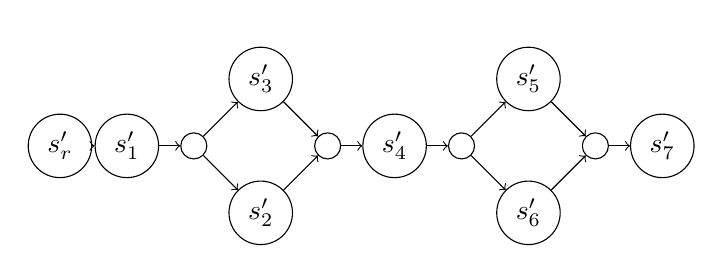
\begin{tikzpicture}[scale=0.85]
    \node[draw, circle] (node1) at (0,0) {$s^\prime_r$};
    \node[draw, circle] (node2) at (1,0) {$s^\prime_1$};
    \node[draw, circle] (node3) at (2,0) {$\timesOperator$};
    \node[draw, circle] (node4) at (3,-1) {$s^\prime_2$};
    \node[draw, circle] (node5) at (3,1) {$s^\prime_3$};
    \node[draw, circle] (node6) at (4,0) {$\timesOperator$};
    \node[draw, circle] (node65) at (5,0) {$s^\prime_4$};
    \node[draw, circle] (node7) at (6,0) {$\plusOperator$};
    \node[draw, circle] (node8) at (7,1) {$s^\prime_5$};
    \node[draw, circle] (node9) at (7,-1) {$s^\prime_6$};
    \node[draw, circle] (node10) at (8,0) {$\plusOperator$};
    \node[draw, circle] (node11) at (9,0) {$s^\prime_7$};
    % Text on top
    \node[above] at (node1.north) { \footnotesize$\instanceChartAnnotation$};
    \node[above] at (node2.north) { \footnotesize$\instanceChartAnnotation$};
    \node[above] at (node3.north) {};
    \node[above] at (node4.north) { \footnotesize$\instanceChartAnnotation$};
    \node[above] at (node5.north) { \footnotesize$\instanceChartAnnotation$};
    \node[above] at (node65.north) { \footnotesize$\instanceChartAnnotation$};
    \node[above] at (node8.north) { \footnotesize$\instanceChartAnnotation$};
    \node[above] at (node9.north) { \footnotesize$\instanceChartAnnotation$};
    \node[above] at (node11.north) { \footnotesize$\instanceChartAnnotation$};
    % Connection
    \draw[->] (node1) -- (node2);
    \draw[->] (node2) -- (node3);
    \draw[->] (node3) -- (node4);
    \draw[->] (node3) -- (node5);
    \draw[->] (node5) -- (node6);
    \draw[->] (node4) -- (node6);
    \draw[->] (node6) -- (node65);
    \draw[->] (node65) -- (node7);
    \draw[->] (node7) -- (node8);
    \draw[->] (node7) -- (node9);
    \draw[->] (node8) -- (node10);
    \draw[->] (node9) -- (node10);
    \draw[->] (node10) -- (node11);
  \end{tikzpicture}
  \caption{Service composition instance}
  \label{fig:service_composition_instance}
\end{figure}
